\chapter{Methodology}
\section{Datasets Description}
\subsection{TREC News Dataset}
\cite{RN19} This collection contains 608,180 news articles and blog posts ranging from January 2012 to August 2017. For the purpose of testing our hypothesis, we use a sample of $\mathtt{\sim}$ 21000 documents with approximately $\mathtt{\sim}$ 2400 relevant documents. However, this has been done only for time-based index due to scalability and resource constraints. And the term age is still calculated considering the entire corpus and does not affect the algorithmic logic. The dataset is in JSON file format containing following fields: id, URL, title, author, published date, article text broken into paragraphs, caption and author bio. We have created three indices in our Elasticsearch server, one which contains all this dataset, as present in the given JSON file, with a regular mapping. Second index containing the updated term weight parameter containing a time normalized term weight to be used later in relevance score calculation and retrieval. And a third index containing the USE text embedding vector field along with the term weight parameter.

For testing the results, and setting up a ground truth for the system, we have used TREC – 2018 news background linking task \cite{RN20}. This task is about fetching the background related news articles providing the context for the main article. The intuition behind this is the reader should get all the relevant information about the searched topic from the best possible source \cite{Huang2018trec}. For example, if the search topic headline is "How major U.S. cities and transit systems are reacting to the Brussels attacks", then the related relevant article would be "Transportation agencies across the U.S. step up security in wake of Paris attacks" or "Islamic State claims responsibility for the Brussels attacks". There are 50 such queries given to us, with the following fields, Document number, ID, URL. This is used as an input query file to our information retrieval system. Another data file is given which contains the most relevant results for each given query in the input document. These results are human checked and can be considered as the ground truth for our experiment. This file contains the following fields: Document Number, Document ID, Gain Value (which is defined as $2^r$, where r is relevance scale ranging from 0 to 4). Document number referred in this file is same as the one given in the input queries file. So, this file sets up the ground truth for the given set of queries, the documents which are relevant to each query and scale of relevancy for these documents.
\textit{Figure} \ref{fig:trec-news-dataset} shows the glimpse of the dataset and its structure and \textit{Table} \ref{tab:trec-ground-truth} shows the relevant gold standard relevance values given to us.

\begin{table}[h!]
    \centering
    \begin{tabular}{|c|c|c|}
    \hline
    \textbf{query number} & \textbf{id} & \textbf{Relevance ($2^r$)}\\
    \hline
    321 & 00f57310e5c8ec7833d6756ba637332e & 16\\
    321 & 02ae7136-006d-11e3-9711-3708310f6f4d & 2\\
    321 & 049739753ce2e539d8dc2165daaf6aa6 & 4\\
    \hline
    \end{tabular}
    \caption{TREC News gold standard snapshot}
    \label{tab:trec-ground-truth}
\end{table}

\begin{figure}
    \centering
    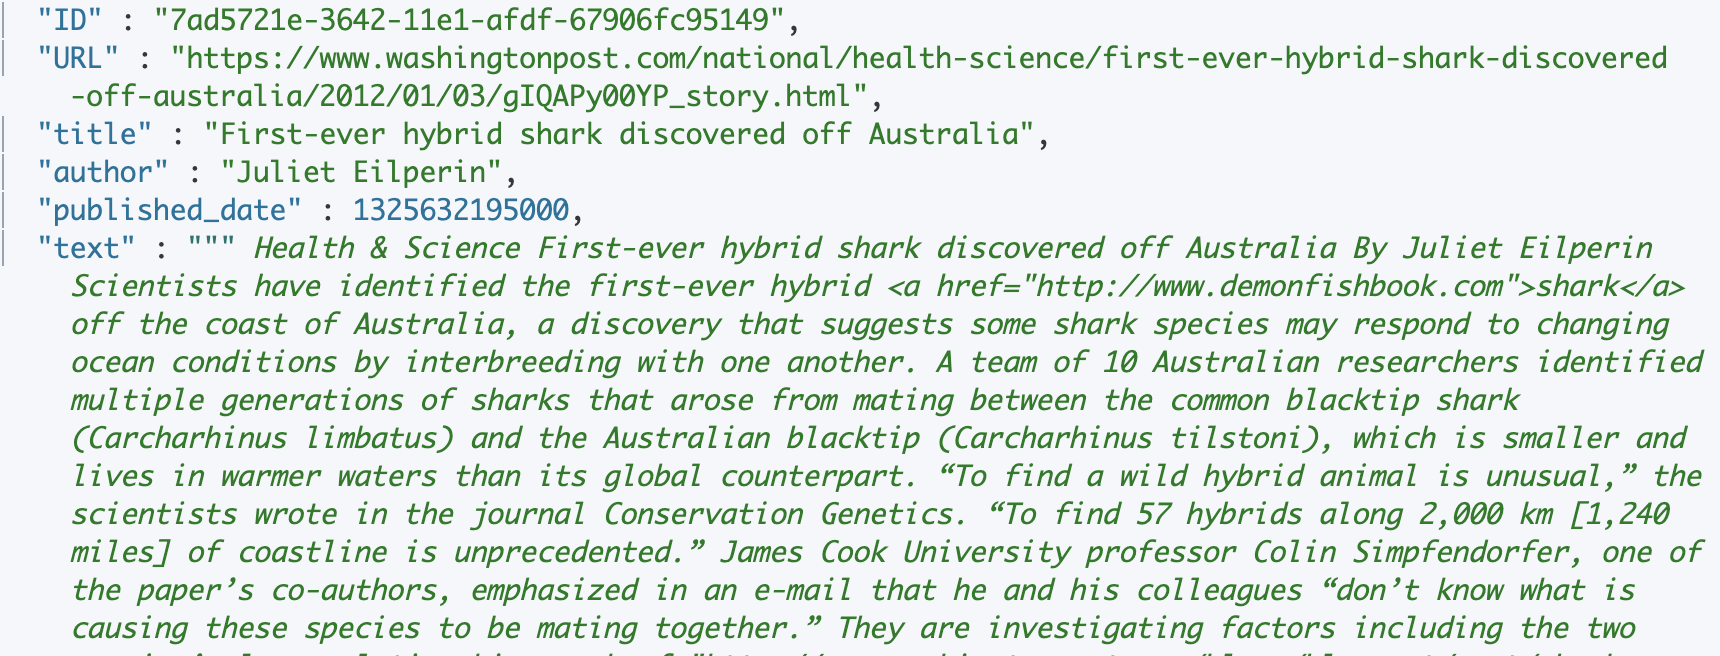
\includegraphics[width=140mm, scale=0.7] {trec-news-dataset-structure.png}
    \caption{TREC News dataset structure }
    \label{fig:trec-news-dataset}
\end{figure}

\subsection{Web AP Dataset} 

\cite{RN30, RN31} This collection contains 8027 articles from the web, which are answers to 82 TREC queries. The dataset is a subset of 2004 TREC Terabyte track Gov2 dataset \cite{clarke2004overview} along with the test query topics specified in the track. This dataset is cleaned and contains relevant passages for the 82 test queries specified in the ground truth. Length of an average passage in this dataset is 45 words.
\begin{figure}[h!]
    \centering
    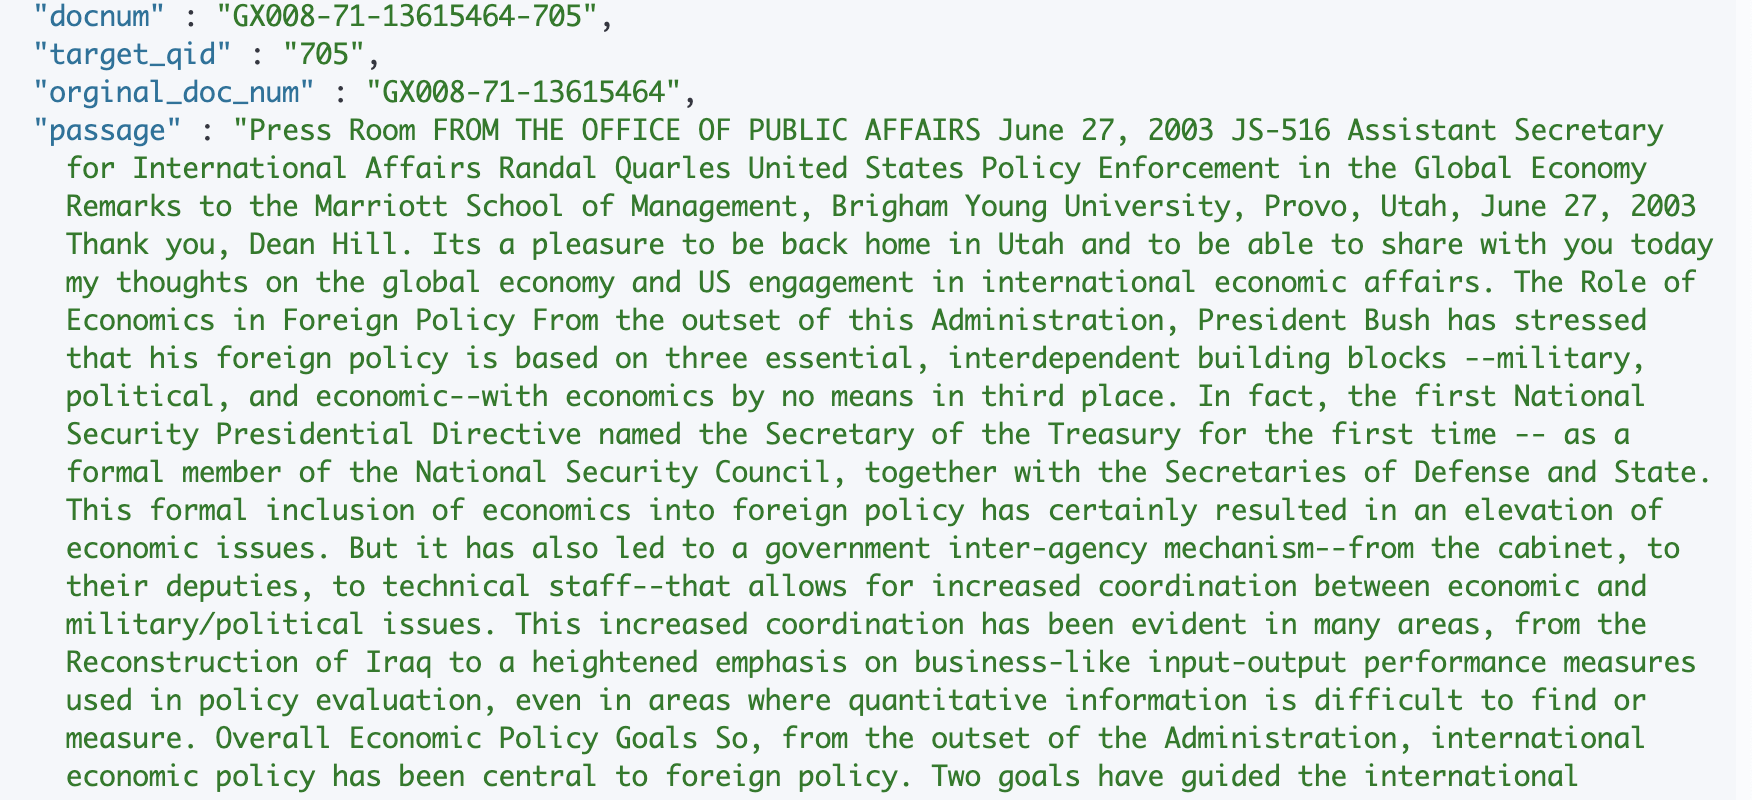
\includegraphics[width=140mm, scale=07]{WebAP-dataset-structure.png}
    \caption{Web AP dataset structure }
    \label{fig:web-ap-dataset}
\end{figure}

The dataset is in JSON file format containing the following fields: unique document id, target question id, and passage. We have created three indices from this dataset, one containing the data as it is given in JSON file. Second index containing the updated term weight parameter as the time-normalized factor. And the third index with dense vectors for USE embedding along with the time-normalized factor. We are given ground truth results for the given set of 82 queries as set of 50 most relevant results. The results are given as question\_id, document number and relevance as ranked from 1 to 50. \textit{Figure} \ref{fig:web-ap-dataset} shows the glimpse of the dataset and its structure.

One of the sample query used in the evaluation is given in the following form: \\
\textit{
$<$query$>$	\\	
$<$title$>$\\	
$<$docno$>$DOCNO701$</$docno$>$.\\
$<$tag$>$U.S. oil industry history $</$tag$>$\\
$</$title$>$\\	
$<$desc$>$\\	
$<$docno$>$DOCNO701$</$docno$>$.\\
$<$tag$>$ Describe the history of the U.S. oil industry $</$tag$>$\\
$</$desc$>$	\\
$</$query$>	$\\	
}

And table \ref{tab:web-ap-gold} shows a snapshot of the gold standard relevance results for the above mentioned query:
\begin{table}[h!]
    \centering
    \begin{tabular}{|c|c|c|}
    \hline
         \textbf{Number }& \textbf{docnum} & \textbf{relevance}  \\
         \hline
         701 & GX268-35-11839875 & 1\\
         701 & GX262-28-10569245 & 2 \\
         701 & GX238-57-4348848	& 3	\\
         701 & GX231-53-10990040 &	4\\	
         \hline
    \end{tabular}
    \caption{Web AP Gold standard relevance}
    \label{tab:web-ap-gold}
\end{table}


\subsection{CiteULike Dataset}
\cite{DBLP:conf/ijcai/WangCL13} This dataset is collected from CiteULike and Google Scholar and contains 17013 documents. CiteULike was a service that allowed people to create their personal article or paper collection. The dataset is given in CSV file format with the following fields: docid (unique document id), title (lower case title), raw\_title(original title of the research paper), and abstract. We have created three indices from this dataset, one containing the data as it is and another one containing the time normalized term weight parameter and a third index containing the dense vectors based on USE encoding along with the term age metric.

We are given another file in this dataset, that contains the referenced articles for every document. This serves as our problem statement to develop a research paper recommender system. The input for this will be the title of the paper and the expected results would be the referenced article for this paper. Since the references are given for every article, and it will make the evaluation biased and difficult for aggregating the results. In order to fix this issue, we have randomly selected 116 test topics having exactly 10 citations to be used as our ground truth. 
\textit{Figure} \ref{fig:citeulike-dataset} shows the glimpse of the dataset and its structure.

\begin{figure}[h!]
    \centering
    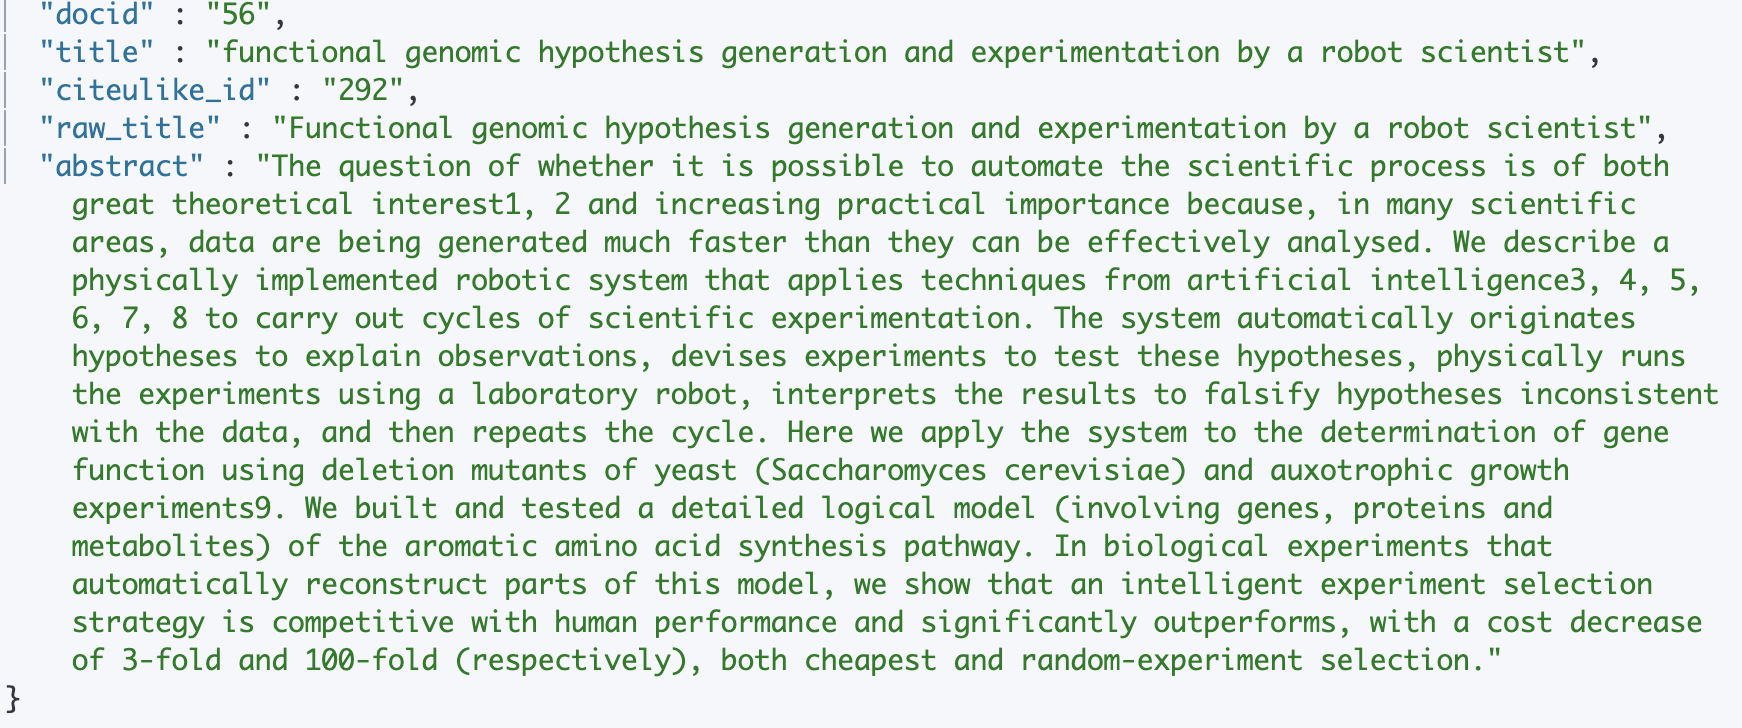
\includegraphics[width=140mm, scale=0.7]{cite-u-like-dataset-structure.png}
    \caption{CiteULike dataset structure }
    \label{fig:citeulike-dataset}
\end{figure}

\section{Evaluation Metrics}
\subsection{Precison@10}
Precision is defined as the number of relevant results in retrieved result set. Generally, precision is calculated for top K number of results, given as P@K. This evaluates the number of relevant results fetched in the top K number of results. We have tested our IR system on given set of 50 queries(for TREC News), 82 queries(for Web AP) and 116 queries(for CiteUlike) , so we calculate the average precision which takes the mean of the precision calculated for all the given queries. We have taken the value of K as 10, so we test the relevance of top 10 results in our scenario. We have calculated the precision value for top 10 fetched results on the given set of input queries and take an average of the results for comparison.
We have calculated the precision value for top 10 fetched results on the given set of input queries and take an average of the results for comparison.

\subsection{Recall (TREC News dataset only)}
For calculating the recall, we have considered the queries having less than 100 results, in case of TREC news. And then recall is calculated as the number of relevant retrieved document divided by the number of relevant documents present in the index. For other datasets, since the number of relevant results is fixed, so the value of precision and recall remains the same.

\subsection{F1 Score (TREC News dataset only)}
Since F1 score uses both the precision and recall values, so for calculating the precision scores, we have used the same results from the recall measure and used a fixed denominator as the number of retrieved results (100 in our case). Formula used for F1 score is given as:
	\begin{equation}
	    F1= 2*(Precision*Recall)/(Precision+Recall)
	\end{equation}
   
\subsection{NDCG@10 Score}
This is a measure of ranking quality. This is based on the assumption that more relevant documents are placed higher in the result list. In calculating DCG, higher relevant result placed at a lower position is penalized by the log value of proportional to the position. DCG is calculated at specific rank position p, given by 
	\begin{equation}
	DCG_{p} = \sum{i=1}{p} rel_{i}/\log_{2}(i+1)
	\end{equation}
where, $rel_{i}$ is the relevance score of a document at position $i$. And NDCG is calculated by considering the DCG of ideal order along with the DCG values and is given by
\begin{equation}
    nDCG_{p} = DCG_{p}/IDCG_{p}
\end{equation}
where $IDCG_{p}$ is the ideal DCG values at position p. This is considered from the ground truth or from human verified results, that specify the ranking of results they prefer for relevance.
We have taken the value at position 10 and calculated the nDCG for the top 10 results. We have fetched the results for given set of queries, so we calculate the average nDCG for both set of algorithms and compare the results.